%===================================================================================
\subsection{CU19 Registrar repositorio proyecto}
{
\justify
\color{blue}{\textbf{Objetivo}}
}

%------------------------------------------------------------------
\justify
En esta pantalla permite al Lider proyecto registrar el repositorio en donde se esta versionando el proyecto.
%------------------------------------------------------------------
{
\justify
\color{blue}{\textbf{Diseño}}
}
%-------------------------------------------------------------------------------
\justify
En la figura \ref{fig:IU19} se muestra la pantalla, en donde el Lider de proyecto podrá registrar el repositorio en donde se esta versionando el proyecto.

\begin{figure}[htb]
\centering
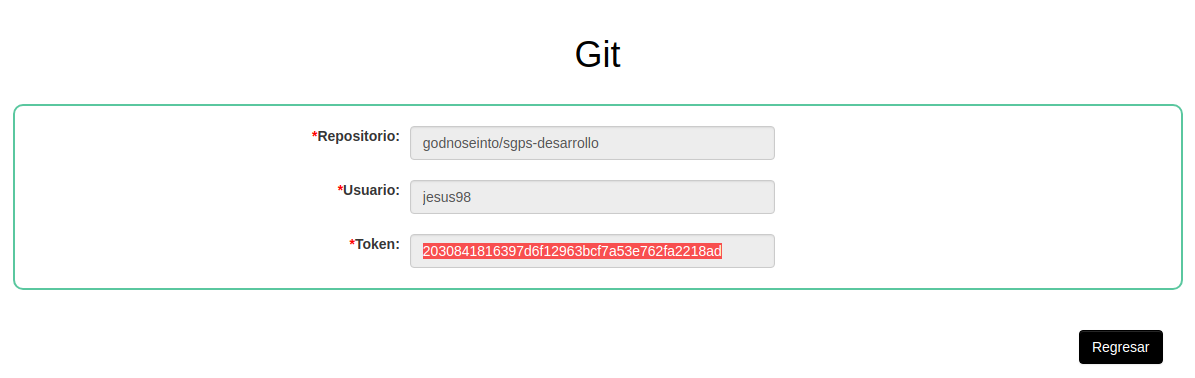
\includegraphics[width=0.8\textwidth]{./images/cu19-registrar-repositorio-proyecto.png}
\caption{Registrar repositorio proyecto.} \label{fig:IU19}
\end{figure}